\documentclass[twocolumns,landscape]{article}
%\usepackage[usenames,dvipsnames]{xcolor}
\usepackage{tkz-fct}
\begin{document}

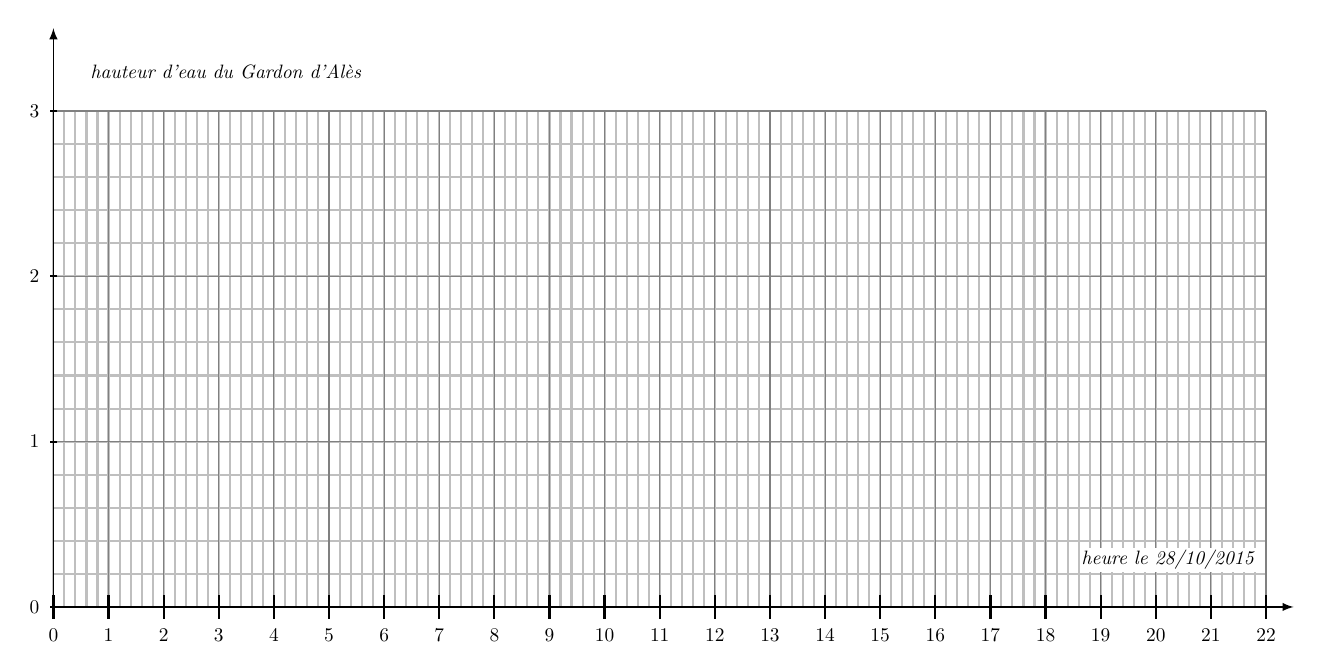
\begin{tikzpicture}[scale=0.7,yscale=3,every node/.style={scale=0.7}]
\tkzInit[xmax= 22,xstep=1,ymax=3,ystep=1]
\tkzGrid[sub]
\tkzDrawX[label={\textit{heure le 28/10/2015}},above left=18pt,fill=white]
\tkzLabelY
\tkzLabelX
\tkzDrawY[label={\textit{hauteur d'eau du Gardon d'Al\`es}},below right=18pt]

\draw plot[smooth] file {ales.table};
\end{tikzpicture}



\end{document}

%\begin{tikzpicture}
%\tkzInit[xmin=-5,xmax=5,ymax=2]
%\tkzGrid
%\tkzAxeXY
%\tkzFct[color=red]{2*x**2/(x**2+1)}
%\end{tikzpicture}
%
%\begin{tikzpicture}[scale=1.25]
%\tkzInit[xmin=-5,xmax=5,ymax=7]
%\tkzGrid
%\tkzAxeXY
%%\tkzFct[color=red]{2*x**2/(x**2+1)}
%\tkzFct[{-(},color=red,samples=2,domain =-1:2]{(8-1.5*\x)/2}
%\end{tikzpicture}
%
%\begin{tikzpicture}[scale=3]
%\tkzInit[xmax=5,ymax=2]
%\tkzGrid[sub]
%\tkzAxeXY
%\tkzFct[samples=400,domain=.5:5]{1/x}
%\end{tikzpicture}